\section{Unified IBM and GFM Numerical Method}

\subsection{Governing equations}

Assuming a collisionless plasma, the evolution of the distribution function for particle species $s$ is governed by the Vlasov equation:
\begin{equation}
	\label{eq:vlasov}
	\partial_t f_s + \mathbf{v} \cdot \nabla_{\mathbf{x}} f_s + \left(\frac{q_s}{m_s}\mathbf{E}\right)\cdot \nabla_{\mathbf{v}} f_s = 0.
\end{equation}

The \textit{Vlasolver} solves the Vlasov--Poisson system by coupling a kinetic solver for Eq.~\eqref{eq:vlasov} with a field solver for the Poisson equation.

\subsection{Unified coupling framework}

We introduce a cell-centered Cartesian mesh (Fig.~\ref{fig:unified_mesh}), which is shared by both the Vlasov and Poisson solvers. As illustrated in Fig.~\ref{fig:unified_mesh}, both the distribution function and the electrostatic potential are defined at cell centers, enabling a consistent and efficient data exchange between the two solvers.

\begin{figure}[htbp]
	\centering
	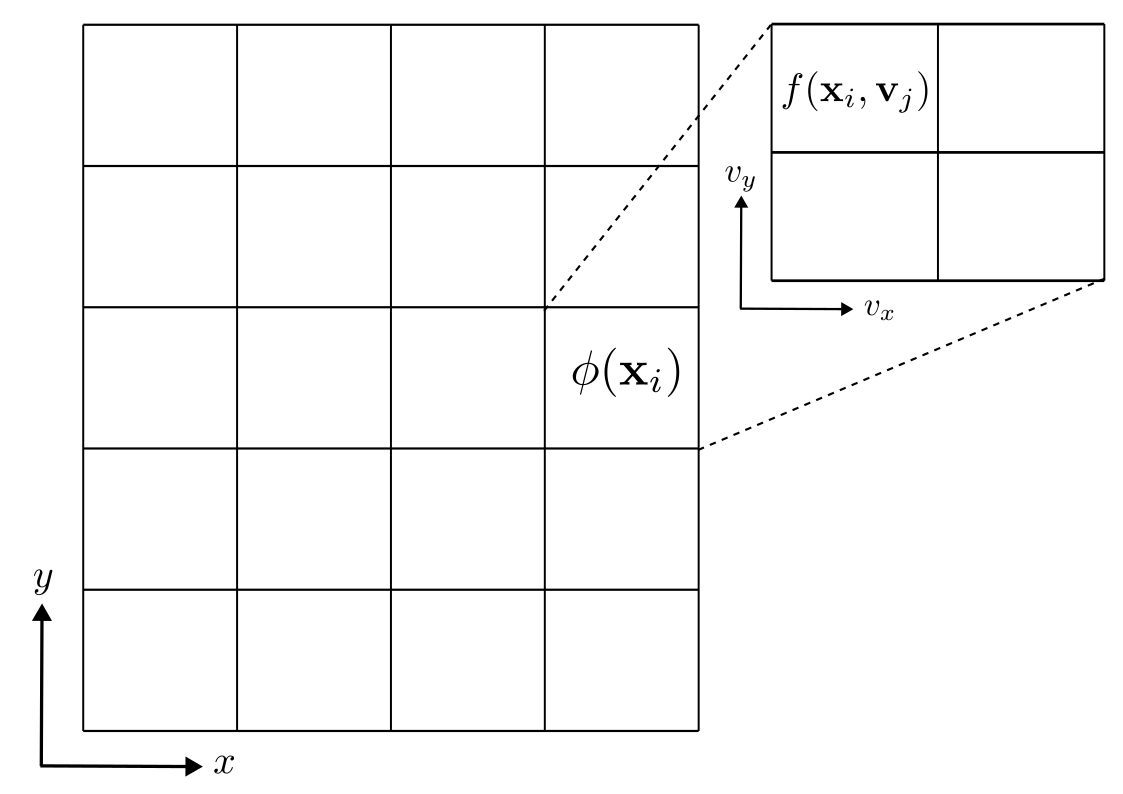
\includegraphics[width=0.6\textwidth]{figures/unified_mesh.png}
	\caption{Schematic of the unified cell-centered mesh used for both the Vlasov and Poisson solvers.}
	\label{fig:unified_mesh}
\end{figure}

The Vlasov equation is discretized using a semi-Lagrangian scheme based on the positive flux-conservative (PFC) formulation. The primary unknown is the cell-averaged distribution function:
\begin{equation}
	f_{ij}^n = \frac{1}{\Delta x \Delta v}
	\int_{x_{i-1/2}}^{x_{i+1/2}}
	\int_{v_{j-1/2}}^{v_{j+1/2}}
	f(\mathbf{x}, \mathbf{v}, t^n)\, \mathrm{d}x\, \mathrm{d}v.
\end{equation}

The scheme advances these cell averages directly, ensuring conservation and positivity without explicitly evaluating the integrals during time evolution.

The electrostatic potential is computed by solving the Poisson equation using a finite-difference method on the same mesh. The charge density is obtained from velocity moments of the distribution function:
\begin{equation}
	\rho(\mathbf{x}) = \sum_s q_s \int f_s(\mathbf{x}, \mathbf{v})\, \mathrm{d}\mathbf{v}.
\end{equation}

The overall coupling procedure is illustrated in Fig.~\ref{fig:coupling_scheme}. At each time step, the Vlasov solver updates the distribution function using the electric field, while the Poisson solver computes the electric field from the charge density. This establishes a self-consistent evolution of particles and fields.

\begin{figure}[htbp]
	\centering
	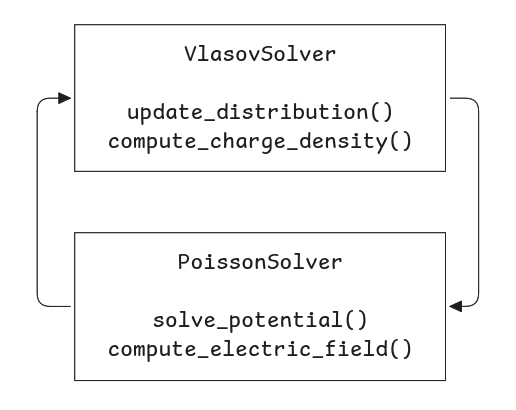
\includegraphics[width=0.75\textwidth]{figures/coupling_scheme.png}
	\caption{Flowchart of the coupling between the Vlasov and Poisson solvers in the Vlasolver framework.}
	\label{fig:coupling_scheme}
\end{figure}

\subsection{Vlasov solver}
A well known second order time integration technique called Strang splitting is applied to the Vlasov equation. This technique splits the Vlasov equation into two advection equations, one in the position space and the other in the velocity space.

\begin{align}
	\label{eq:spatial_advection}
	\partial_t f + \mathbf{v}_s\cdot\grad_{\mathbf{x}} f_s = 0 \\
	\label{eq:velocity_advection}
	\partial_t f + (q_s\mathbf{E}/m_s)\cdot\grad_{\mathbf{v}} f_s = 0
\end{align}

Then update the two advection equations in the following orders:

\begin{equation}
	\label{eq:strang-splitting}
	\begin{aligned}
		f_s^{*}(\mathbf{x}, \mathbf{v})   & = f_s^n(\mathbf{x} - \mathbf{v}_s\Delta t/2, \mathbf{v}),           \\
		f_s^{**}(\mathbf{x}, \mathbf{v})  & = f_s^{*}(\mathbf{x}, , \mathbf{v}- (q_s\mathbf{E}/m_s)\Delta t/2), \\
		f_s^{n+1}(\mathbf{x}, \mathbf{v}) & = f_s^{**}(\mathbf{x} - \mathbf{v}_s\Delta t/2, \mathbf{v}).
	\end{aligned}
\end{equation}

In each step, the advection update is performed using a 3rd-order PFC scheme.

\subsection{PFC scheme for advection update}
Notice that the spatial and velocity advection equations both take the form
\begin{equation}
	\partial_t f + \partial_x(vf) = 0,
	\label{eq:advection_simplified}
\end{equation}
where $v$ denotes as velocity $\mathbf{v}$ in Eq.~(\ref{eq:spatial_advection}) or acceleration $q\mathbf{E}/m$ in Eq.~(\ref{eq:velocity_advection}). A PFC scheme is implemented to solve such advection equation.

On a uniform cell-centered mesh defined on computational domain $[x_{\text{min}}, x_{\text{max}}]$. The cell centers are defined as $x_i = x_{\text{min}} + (i+1/2)\Delta x$, where $\Delta x$ is the cell size. We use $f_i^n=\int_{x_{i-1/2}}^{x_{i+1/2}} f(x,t^n)\dd x/\Delta x$ to denote the average distribution function at the $i$-th cell center and time step $n$.

The PFC scheme updates the distribution function at the next time step, $f_i^{n+1}$, by tracing the characteristic line back to the previous time step, $t^n$,

\begin{equation}
	\int_{x_{i-1/2}}^{x_{i+1/2}} f(x, t^{n+1}) \dd x = \int_{x_{i-1/2} - v\Delta t}^{x_{i+1/2} - v\Delta t} f(x, t^n) \dd x.
	\label{eq:trace_characteristic}
\end{equation}

Meaning that the cell-averaged distribution function at the next time step, $f_i^{n+1}$, can be evaluated by

\begin{equation}
	f_i^{n+1} = f_i^n + F_{i-1/2} - F_{i+1/2}.
	\label{eq:distribution_update}
\end{equation}
where $F_{i-1/2} = \int_{x_{i-1/2} - v\Delta t}^{x_{i-1/2}} f(x, t^n) \dd x/\Delta x$ and $F_{i+1/2}=\int_{x_{i+1/2} - v\Delta t}^{x_{i+1/2}} f(x, t^n) \dd x/\Delta x$ are the fluxes through the cell left and right interfaces.

The flux can approximated by a 3rd-order scheme,
\begin{equation}
	F_{i+1/2} = \begin{cases}
		\abs{\varphi}\left( f_{j}^n + \frac{1}{6}(2 - \abs{\varphi})(1-\abs{\varphi})(f_{j+1}^n - f_{j}^n) + \frac{1}{6}(1 - \abs{\varphi})(1+\abs{\varphi})(f_{j}^n - f_{j-1}^n)\right), & \varphi > 0, \\
		\abs{\varphi}\left( f_{j}^n + \frac{1}{6}(2 - \abs{\varphi})(1-\abs{\varphi})(f_{j}^n - f_{j-1}^n) + \frac{1}{6}(1 - \abs{\varphi})(1+\abs{\varphi})(f_{j+1}^n - f_{j}^n)\right), & \varphi < 0.
	\end{cases}
	\label{eq:flux_3rd_order}
\end{equation}
where $\varphi = v\Delta t/\Delta x$ is related to CFL number, and $j = i - \lfloor\varphi\rfloor$.

To preserve positivity of the distribution function, a flux limiter described in \cite{liu2021conservative} is applied to the flux,
\begin{equation}
	\hat{F}_{i+1/2} = L_{i+1/2} \left( F_{i+1/2} - f_{i+1/2} \right) + f_{i+1/2}.
	\label{eq:modified_flux}
\end{equation}

The $L_{i+1/2} = \min(L_i^r, L_{i+1}^l)$, where
\begin{equation}
	L_i^l =
	\begin{cases}
		\min\left(1, \delta_i^k/d_{i-1/2} \right), & d_{i-1/2} < 0 \text{ and } d_{i+1/2} < 0,     \\
		\delta_i^k/(d_{i-1/2} - d_{i+1/2}),        & d_{i-1/2} d_{i+1/2} < 0 \text{ and } p_i < 0, \\
		1,                                         & \text{else},
	\end{cases}
	\label{eq:flux_limiter_left}
\end{equation}

\begin{equation}
	L_i^r =
	\begin{cases}
		\min\left(1, -\delta_i^k/d_{i+1/2} \right), & d_{i-1/2} \ge 0 \text{ and } d_{i+1/2} > 0,   \\
		\delta_i^k/(d_{i-1/2} - d_{i+1/2}),         & d_{i-1/2} d_{i+1/2} < 0 \text{ and } p_i < 0, \\
		1,                                          & \text{else},
	\end{cases}
	\label{eq:flux_limiter_right}
\end{equation}

where $f_{i+1/2} = \varphi f_i^n$ is the first order flux, and $\epsilon_{i+1/2}\in[0,1]$ is the positivity-preserving limiter to ensure the positivity of the function $f_{i}^{n+1}$ in Eq.~(\ref{eq:distribution_update}). We denote $d_{i\pm1/2} = F_{i\pm1/2} - f_{i\pm1/2}$ and $p_i = d_{i-1/2} - d_{i+1/2} -\delta_i^n$.

Finally, the new update scheme for the distribution function is
\begin{equation}
	f_i^{n+1} = f_i^n + \hat{F}_{i -1/2} - \hat{F}_{i+1/2}.
	\label{eq:final_update}
\end{equation}

\subsection{Immersed boundary treatment for the Vlasov solver}

The computational domain is partitioned into fluid, solid, and ghost cells. As shown in Fig.~\ref{fig:ibm_2nd_order}, ghost cells are solid cells adjacent to the interface that are used to enforce boundary conditions.

\begin{figure}[htbp]
	\centering
	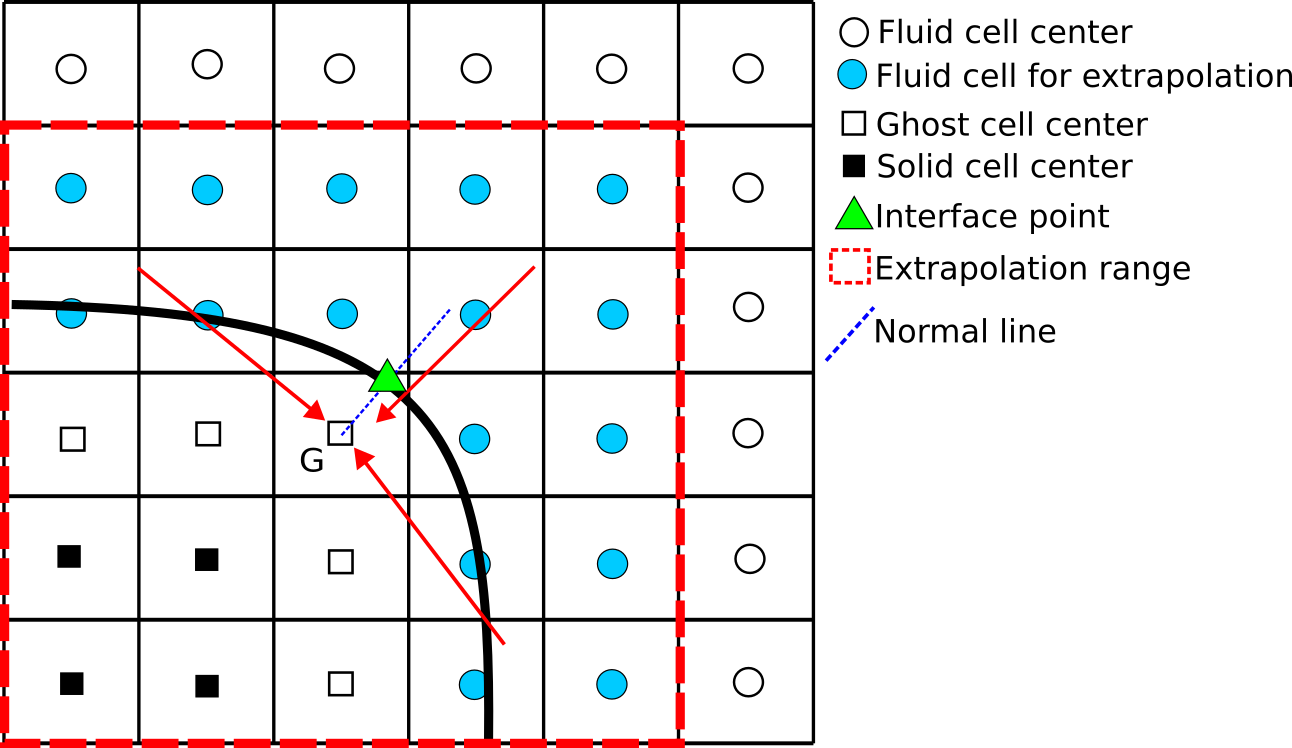
\includegraphics[width=0.6\textwidth]{figures/immersed_boundary_2nd_order.png}
	\caption{Illustration of cell classification and interface representation in the immersed boundary method.}
	\label{fig:ibm_2nd_order}
\end{figure}

The interface is implicitly represented, and its intersection with grid lines defines interface points $\mathbf{x}_I$. At each interface point, the outward normal vector $\mathbf{n}$ is computed to distinguish inflow and outflow directions in velocity space.

The boundary condition is imposed directly on the distribution function at interface points. The treatment depends on the sign of $\mathbf{v}\cdot \mathbf{n}$:

\begin{itemize}
	\item \textbf{Outflow ($\mathbf{v}\cdot \mathbf{n} < 0$):}
	      The distribution function is extrapolated from interior fluid values.

	\item \textbf{Inflow ($\mathbf{v}\cdot \mathbf{n} > 0$):}
	      A fully absorbing boundary condition is imposed, i.e., $f(\mathbf{x}_I, \mathbf{v}) = 0$.
\end{itemize}

This directional treatment ensures consistency with the kinetic transport mechanism and avoids unphysical reflections at the boundary.

Once the interface values are determined, ghost-cell values are reconstructed to complete the numerical stencil. As illustrated in Fig.~\ref{fig:ibm_2nd_order}, the ghost value is obtained by extrapolation using the nearby fluid cells.

Given a range for extrapolation (Fig.~\ref{fig:ibm_2nd_order}), the coefficients, $c_0$, $c_1$ and $c_2$ are determined by the distribution function at near-by fluid cells, which are selected based on the shape of the immersed object. Then solving a least-square problem we can obtain the coefficients,

\begin{equation}
	\min_{c_0,c_1,c_2} \sum_{k=1}^{N_F} (c_0 + c_1x_k + c_2y_k - f_k)^2
	\label{eq:least_square_matrix}
\end{equation}
where $N_F$ is the number of near-by fluid cells in the extrapolation range, and $f_k$ is the distribution function at the $k$-th near-by fluid cell.

\begin{equation}
	f(\mathbf{x}_G, \mathbf{v}, t) = \begin{cases}
		0                              & , \mathbf{v}\cdot\mathbf{n} > 0, \\
		\max(c_0 + c_1x_G + c_2y_G, 0) & , \mathbf{v}\cdot\mathbf{n} < 0.
	\end{cases}
	\label{eq:extrapolation}
\end{equation}

\subsection{Second-order ghost-fluid treatment for the Poisson equation}

We consider the elliptic interface problem on a 2D domain $\Omega \subset \mathbb{R}^2$:
\begin{align}
	\nabla \cdot (\epsilon \nabla \phi) & = f \quad \text{in } \Omega \setminus \Gamma, \\
	[\phi]                              & = a \quad \text{on } \Gamma,                  \\
	[\epsilon \partial_n \phi]          & = b \quad \text{on } \Gamma,
\end{align}
where $\Gamma$ is an interface separating $\Omega$ into $\Omega^+$ and $\Omega^-$, and $[q] = q^+ - q^-$ denotes the jump. The unit normal vector is computed by
\begin{align}
	\mathbf{n} = \frac{\nabla \eta}{|\nabla \eta|}.
\end{align}

Throughout the discussion, we assume $\epsilon$ is piecewise constant and $a,b$ are given functions defined on the interface. The normal vector components $n_x$ and $n_y$ are approximated by fourth-order central differences of the level set function $\eta$.

\subsubsection{Finite Difference Discretization}

Away from the interface, the equation is discretized using standard second-order central differences:
\begin{equation}
	\begin{aligned}
		 & \frac{1}{\Delta x}
		\left[
			\epsilon_{i+\frac{1}{2},j} \frac{\phi_{i+1,j} - \phi_{i,j}}{\Delta x}
			-
			\epsilon_{i-\frac{1}{2},j} \frac{\phi_{i,j} - \phi_{i-1,j}}{\Delta x}
		\right]               \\
		+
		 & \frac{1}{\Delta y}
		\left[
			\epsilon_{i,j+\frac{1}{2}} \frac{\phi_{i,j+1} - \phi_{i,j}}{\Delta y}
			-
			\epsilon_{i,j-\frac{1}{2}} \frac{\phi_{i,j} - \phi_{i,j-1}}{\Delta y}
			\right] = f_{i,j}.
	\end{aligned}
\end{equation}

\subsubsection{Interface Treatment via Boundary Condition Capturing}

For each grid point $(i,j)$ near the interface, define four directional points:
\begin{align}
	x_R & = (x_i + \theta_R \Delta x, y_j), \quad
	x_L = (x_i - \theta_L \Delta x, y_j),         \\
	x_T & = (x_i, y_j + \theta_T \Delta y), \quad
	x_B = (x_i, y_j - \theta_B \Delta y),
\end{align}
where $\theta \in (0,1]$ gives the fractional distance to the interface, computed from the level set function using quadratic interpolation. For example, if $(x_i, y_j)\in\Omega^-$, then

\begin{equation}
	\theta_R = \begin{cases}
		1                                                                                   & , \eta_{i+1,j}\eta_{i,j} > 0 \\
		\frac{-D_x^0\eta + \sqrt{(D_x^0\eta)^2 - 4(D_{xx}^0\eta)\eta_{i,j}}}{2D_{xx}^0\eta} & , \eta_{i+1,j}\eta_{i,j} < 0
	\end{cases},
	\label{eq:theta_computation}
\end{equation}
where $D_{xx}^0\eta = (\eta_{i-1,j}-2\eta_{i,j}+\eta_{i+1,j})/2$ and $D_x^0\eta = (\eta_{i+1,j}-\eta_{i-1,j})/2$. For $\mathbf{x}_L, \mathbf{x}_T$ and $\mathbf{x}_B$, and the case where $(x_i, y_j)\in\Omega^+$ are computed similarly.


\subsubsection{Second-Order Interface Reconstruction}

At an interface point (e.g. $\mathbf{x}_R$), denote the one-sided values by $\phi^-_R$ and $\phi^+_R$. These are determined by enforcing:
\begin{align}
	[\phi](\mathbf{x}_I)            & = a_I, \\
	[\epsilon \phi_n](\mathbf{x}_I) & = b_I,
\end{align}
where $a_I$ is approximated by cubic interpolation of $b_{i-1}, b_{i}, b_{i+1}, b_{i+2}$ and so is $b_I$.

\subsubsection{Modified Discrete Operator}

The final discrete equation at $(i,j)$ becomes:
\begin{equation}
	\begin{aligned}
		 & \left[
			\epsilon_{i+\theta_R/2,j} \frac{\phi_R - \phi_{i,j}}{\theta_R \Delta x}
			-
			\epsilon_{i-\theta_L/2,j} \frac{\phi_{i,j} - \phi_L}{\theta_L \Delta x}
			\right]
		\left/ \left(\frac{\theta_R+\theta_L}{2} \Delta x\right) \right. \\
		+
		 & \left[
			\epsilon_{i,j+\theta_T/2} \frac{\phi_T - \phi_{i,j}}{\theta_T \Delta y}
			-
			\epsilon_{i,j-\theta_B/2} \frac{\phi_{i,j} - \phi_B}{\theta_B \Delta y}
			\right]
		\left/ \left(\frac{\theta_T+\theta_B}{2} \Delta y\right) \right.
		= f_{i,j},
	\end{aligned}
	\label{eq:modified_poisson}
\end{equation}
where $\phi_R, \phi_L, \phi_T, \phi_B$ are either:
\begin{itemize}
	\item standard cell values (no interface crossing), or
	\item interface values expressed in terms of neighboring cell values.
\end{itemize}

\subsubsection{Solving for Interface Ghost Fluid Values}

In 2D, the normal derivative jump condition $[\epsilon \phi_n]$ are expressed in terms of Cartesian derivatives as $[\epsilon \phi_x]$ and $[\epsilon \phi_y]$. We have two different approaches to compute $[\epsilon \phi_x]$ and $[\epsilon \phi_y]$: One from the normal/tangential jumps and the other from a second-order polynomial reconstruction of $\phi$ in $\Omega^-$. By equating these two different discretizations, we can solve for the unknown interface values $\phi_R^-, \phi_L^-, \phi_T^-, \phi_B^-$.

In 2D, jumps in Cartesian derivatives are related to normal/tangential jumps:
\begin{equation}
	\begin{aligned}
		[\epsilon \phi_x] & = [\epsilon \phi_n] n_x - [\epsilon \phi_\tau] n_y                               \\
		                  & = [\epsilon \phi_n] n_x - [\epsilon]\phi_\tau^- n_y - \epsilon^+ [\phi]_\tau n_y \\
		                  & = [\epsilon \phi_n] n_x - [\epsilon]\phi_\tau^+ n_y - \epsilon^- [\phi]_\tau n_y
		\label{eq:poisson_derivative_jump_x}
	\end{aligned}
\end{equation}
and
\begin{equation}
	\begin{aligned}
		[\epsilon \phi_y] & = [\epsilon \phi_n] n_y + [\epsilon \phi_\tau] n_x                                \\
		                  & = [\epsilon \phi_n] n_y + [\epsilon]\phi_\tau^- n_x + \epsilon^+ [\phi]_\tau n_x  \\
		                  & = [\epsilon \phi_n] n_y + [\epsilon]\phi_\tau^+ n_x + \epsilon^- [\phi]_\tau n_x,
		\label{eq:poisson_derivative_jump_y}
	\end{aligned}
\end{equation}
where the following identity was used:
\begin{equation}
	[pq] = [p]q^- + p^+[q].
\end{equation}
Since $[\phi] = a$, so $[\phi]_\tau \approx a_\tau$. The discretization of $a_\tau$ is obtained by applying fourth-order central differences to the $a$,
\begin{equation}
	(a_\tau)_{i,j} = -(D_xa)(n_y)_{i,j} + (D_ya)(n_x)_{i,j},
\end{equation}
where $D_xa=(-a_{i+2,j}+8a_{i+1,j}-8a_{i-1,j}+a_{i-2,j})/12\Delta x$, $D_ya=(-a_{i,j+2}+8a_{i,j+1}-8a_{i,j-1}+a_{i,j-2})/12\Delta y$.

Let $\mathbf{x}_{\text{ext}} = (x_{\text{ext}},y_{\text{ext}})$ be any of the four points $(x_{i-1}, y_{j-1}), (x_{i+1}, y_{j-1}), (x_{i-1}, y_{j+1}),(x_{i+1}, y_{j+1})$ belonging to $\Omega^-$. $\phi_{\text{ext}}$ refers to the value of $\phi$ at $\mathbf{x}_{\text{ext}}$. Then, consider a quadratic polynomial $P(x,y) = Ax^2 + Bxy + Cy^2 + Dx + Ey + F$ that satisfies that interpolates:
\begin{equation}
	\begin{aligned}
		P(\mathbf{x}_T)            & = \phi_T^-,          \\
		P(\mathbf{x}_B)            & = \phi_B^-,          \\
		P(\mathbf{x}_L)            & = \phi_L^-,          \\
		P(\mathbf{x}_R)            & = \phi_R^-,          \\
		P(x_i,y_j)                 & = \phi_{i,j},        \\
		P(\mathbf{x}_{\text{ext}}) & = \phi_{\text{ext}}.
	\end{aligned}
\end{equation}
We can always express the coefficients of polynomial $P$ in terms of $\phi_T^-, \phi_B^-, \phi_L^-, \phi_R^-, \phi_{i,j}, \phi_{\text{ext}}$ by solving the above linear system.

Finally, Eq.~(\ref{eq:poisson_derivative_jump_x}) can be approximated by
\begin{equation}
	[\epsilon \phi_x] \approx [\epsilon \phi_n] n_x - [\epsilon]\left(\grad{P}\cdot\tau\right)n_y - \epsilon^+ a_\tau n_y.
	\label{eq:poisson_derivative_jump_x_geometry}
\end{equation}
In the computation, $b, n_x, n_y, a_\tau$ are approximated by cubic interpolation of quantities defined at mesh cells.

Suppose the interface lies at $\mathbf{x}_{i,j} + \mathbf{x}_R$, then substitute $\phi_L = \phi_{i-1,j}, \phi_T=\phi_{i,j+1}, \phi_B=\phi_{i,j-1}$ into Eq.~(\ref{eq:poisson_derivative_jump_x_geometry}), we can express $[\epsilon \phi_x]$ in terms of $\phi_R^-$ and neighboring cell values. This gives us one approximation of $[\epsilon \phi_x]$ at $\mathbf{x}_R$.

On the other hand, the jump $[\epsilon \phi_x](\mathbf{x}_R)$ by definition is
\begin{equation}
	[\epsilon \phi_x]_R = \eval{\epsilon^+\phi_x^+ - \epsilon^-\phi_x^-}_{\mathbf{x}_R}.
\end{equation}
Therefore, $[\epsilon \phi_x]$ can be approximated by approximating $\phi^+$ and $\phi^-$ using second order finite differences.

By equating the two different approximations of $[\epsilon \phi_x]$,
\begin{equation}
	\eval{\epsilon^+\phi_x^+ - \epsilon^-\phi_x^-}_{\mathbf{x}_R} \approx \eval{[\epsilon \phi_n] n_x - [\epsilon]\left(\grad{P}\cdot\tau\right)n_y - \epsilon^+ a_\tau n_y}_{\mathbf{x}_R},
	\label{eq:equate_derivative_jump}
\end{equation}
we can solve for the unknown interface value $\phi_R^-$. Similarly, by equating the two different approximations of $[\epsilon \phi_x](\mathbf{x}_L)$, we can solve for $\phi_L^-$. Same procedure applies to $\phi_T^-$ and $\phi_B^-$.

Once we obtain the expression of $\phi_R^-, \phi_L^-, \phi_T^-, \phi_B^-$ in terms of neighboring cell values, we can substitute them into the modified discrete operator in Eq.~(\ref{eq:modified_poisson}) to obtain a linear system for $\mathbf{\phi} = [...,\phi_{i,j},...]^T$ at all cells. This linear system is solved by a preconditioned GEMRES solver.
